\documentclass{article}
\setlength{\parindent}{0pt}
\usepackage{amsmath}
\usepackage{slashed}
\numberwithin{equation}{subsection}
\usepackage{amsmath, amsfonts, graphicx, hyperref, xcolor, indentfirst, float, subcaption}
\usepackage[utf8]{inputenc}
\usepackage[italian]{babel}
\linespread{1.2}
\hypersetup{
    colorlinks=false,
    linkbordercolor=white
}
\setlength{\parindent}{0pt}


\begin{document}
\author{Lorenzo Tasca}
\title{Calcolo della suscettività topologica in una teoria di Yang-Mills $\textup{SU}(3)$}
\date{Gennaio 2024}
\maketitle

\begin{abstract}
    L'obiettivo di questo lavoro è di calcolare la suscettività topologica $\chi$ in una teoria di Yang-Mills con gruppo di gauge $\textup{SU}(3)$ (QCD), attraverso una simulazione numerica su reticolo. L'importanza del calcolo di tale quantità risiede nella relazione di Witten-Veneziano, che la lega alla massa del mesone $\eta'$. 
\end{abstract} 
\tableofcontents


\section{Preliminari teorici}

L'$\eta'$ è un mesone pseudoscalare formato da una combinazione di quark up, down e strange e relativi antiquark, a formare un singoletto di colore. Ha una massa di circa $0.957$ GeV, significativamente maggiore di quella degli altri 8 mesoni pseoudoscalari. Tale fatto può essere spiegato solamente guardando al contributo alla massa della particella dovuto alla rottura della simmetria chirale a livello quantistico, quantificato dal meccanismo di Witten-Veneziano. Infatti senza una rottura di tale simmetria, dovrebbe avere la stessa massa del mesone $\eta$, che è circa la metà. La relazione di Witten-Veneziano lega la massa dell'$\eta'$ alle fluttuazioni della carica topologica, in particolare al suo cumulante noto come suscettività. Il calcolo della carica topologica permette pertanto di andare a calcolare la massa della particella da principi primi, andando a confermare la validità di tale meccanismo. In questo lavoro andremo a calcolare la suscettività topologica a partire dalle estrazioni della carica topologica.

\subsection{Teoria di Yang-Mills su reticolo}

L'azione della teoria nel continuo è costruita richiedendo l'invarianza sotto trasformazioni di gauge $\textup{SU}(3)$. È composta da una parte gluonica 
\begin{equation}
    S_G[U]=\frac{1}{2g^2}\int d^4x \, \textup{Tr}[F_{\mu\nu}F_{\mu\nu}],
\end{equation}
dove $U$ è il campo di gauge e si definisce 
\begin{equation}
    F_{\mu\nu}=\partial_\mu U_\nu-\partial_\nu U_\mu-i[U_\mu, U_\nu],
\end{equation}
e da una parte fermionica che si scrive come
\begin{equation}
    \label{azione fermionica}
    S_F[U, \psi, \bar{\psi}]=\int d^4x\, \bar{\psi} [\slashed{D}+m]\psi, 
\end{equation}
dove si è definita la derivata covariante come
\begin{equation}
    \slashed{D}=\gamma_\mu (\partial_\mu-iU_\mu).
\end{equation}
L'azione gluonica può essere discretizzata preservando l'invarianza di gauge anche a passo reticolare finito, andando a definire una derivata discreta come 
\begin{equation}
    \nabla_\mu f(x)=\frac{f(x+\hat{\mu})-f(x)}{a},
\end{equation}
e un tensore di campo analogo al continuo 
\begin{equation}
    F_{\mu\nu}=\nabla_\mu U_\nu-\nabla_\nu U_\mu-i[U_\mu, U_\nu].
\end{equation}
L'azione si scrive come 
\begin{equation}
    S_G=\frac{1}{2g^2}a^4\sum_x \sum_{\mu\nu} \textup{Tr}[F_{\mu\nu}(x)F_{\mu\nu}(x)]+o(a).
\end{equation}
Discretizzare la (\ref{azione fermionica}) risulta più delicato a causa del teorema di Nielsen-Ninomiya, il quale afferma che non è possibile discretizzare l'azione fermionica (mantenendo un buon comportamento del propagatore) senza rompere la simmetria chirale a passo reticolare finito. L'azione classica della QCD nel caso massless infatti è invariante sotto una trasformazione chirale
\begin{equation}
    \label{tras chirale}
    \psi \rightarrow \psi'=e^{-i\beta\gamma_5}\psi, 
\end{equation} 
o equivalentemente 
\begin{equation}
    \{D, \gamma_5\}=0.
\end{equation}
Tale simmetria però non può essere mantenuta su reticolo, ma ciò non risulta problematico in quanto non è una simmetria definente della teoria, ma è una simmetria accidentale.\\ Una possibilità per costruire l'operatore cinetico $D$ su reticolo è di imporre l'equazione di Ginsparg-Wilson
\begin{equation}
    \label{gispasrg wilson}
    \{D, \gamma_5\}=aD\gamma_5D,
\end{equation}
o equivalentemente
\begin{equation}
    \gamma_5D+D\hat{\gamma_5}=0,
\end{equation}
dove abbiamo definito 
\begin{equation}
    \label{gamma5 hat}
    \hat{\gamma_5}=\gamma_5(1-aD).
\end{equation}
A causa della (\ref{gispasrg wilson}) la simmetria chirale è esplicitamente rotta, ma è recuperata nel limite $a\rightarrow 0$.\\La soluzione all'equazione (\ref{gispasrg wilson}) è nota come operatore di Neuberger.\\
L'azione fermionica massless si scrive a questo punto come 
\begin{equation}
    \label{SF su reticolo}
    S_F=a^4\sum_x \bar{\psi}(x)D\psi(x).
\end{equation}
Il funzionale generatore della teoria nel continuo si scrive come 
\begin{equation}
    \label{funzionale}
    Z=\int \left[\mathcal{D}U \mathcal{D}\psi \mathcal{D}\bar{\psi}\right] \, e^{-S_G-S_F}.
\end{equation}
Su reticolo può essere calcolato come un integrale in un numero finito di dimensioni, assieme alla sue funzioni di correlazione. 

\subsection{Carica topologica}

A causa della rottura della simmetria chirale a passo reticolare finito l'azione (\ref{SF su reticolo}) non è più invariante per trasformazioni chirali (\ref{tras chirale}). Risulta essere però essere invariante per una trasformazione chirale modificata, nota come trasformazione di Lüscher
\begin{equation}
    \psi\rightarrow \psi'=e^{i\beta \hat{\gamma_5}}\,\psi,
\end{equation}
\begin{equation}
    \bar{\psi}\rightarrow\bar{\psi}'=\bar{\psi}\,e^{i\beta\gamma_5}.
\end{equation}
Affinché la teoria (quindi le funzioni di correlazione) sia invariante però non è sufficiente che l'azione lo sia, ma deve esserlo anche la misura dell'integrale in (\ref{funzionale}). Questa però non risulta invariante per trasformazioni di Lüscher, infatti effettuando il cambio di variabili grassmaniane si ha che 
\begin{equation}
    \left[\mathcal{D}\psi' \mathcal{D}\bar{\psi}'\right]=\exp\left(-i\beta\,\textup{Tr}\hat{\gamma_5}\right)\left[\mathcal{D}\psi \mathcal{D}\bar{\psi}\right].
\end{equation}
Usando la (\ref{gamma5 hat}) possiamo scrivere che 
\begin{equation}
    \textup{Tr}\hat{\gamma_5}=-a\,\textup{tr}\left(\gamma_5\,D(x,x)\right).
\end{equation}
Definiamo quindi la densità di carica topologica come
\begin{equation}
    \label{top charge density}
    a^4\,q(x)=-\frac{a}{2}\,\textup{tr}\left(\gamma_5\,D(x,x)\right),
\end{equation}
e la carica topologica come 
\begin{equation}
    \label{top charge}
    Q=a^4\sum_x q(x), 
\end{equation}
la quale risulta essere quindi 
\begin{equation}
    Q=\frac{1}{2}\,\textup{Tr}\hat{\gamma_5}
\end{equation}

Si può dimostrare che nel continuo la carica topologica assume solo valori interi, in quanto è la differenza tra il numero di modi a chiaralità positiva e quelli a chiralità negativa.

\subsection{Suscettività topologica}
Definiamo ora la funzione $F$ generatrice dei cumulanti per $Q$. Essa si definisce come 
\begin{equation}
    e^{-F(\theta)}=\left< e^{i\theta Q}\right>=\frac{\int \left[\mathcal{D}U \mathcal{D}\psi \mathcal{D}\bar{\psi}\right] \, e^{-S_G-S_F}e^{i\theta Q}}{\int \left[\mathcal{D}U \mathcal{D}\psi \mathcal{D}\bar{\psi}\right] \, e^{-S_G-S_F}}.
\end{equation}
I suoi cumulanti si scrivono come 
\begin{equation}
    c_n=(-1)^{n+1}\frac{1}{V}\frac{d^{2n}}{d\theta^{2n}}\left.F(\theta)\right|_{\theta=0}, 
\end{equation}
e in particolare il suo secondo cumulante noto come suscettività topologica
\begin{equation}
    \chi=c_1=\frac{1}{V}\frac{d^2}{d\theta^2}\left.F(\theta)\right|_{\theta=0}=a^4\sum_x \left< q(x)q(0)\right>.
\end{equation}
È noto che il secondo cumulante di una distribuzione coincide con la sua varianza. Pertanto 
\begin{equation}
    \chi=\frac{\left< Q^2\right>}{V}.
\end{equation}
Dalle estrazioni di $Q$ possiamo quindi ottenere la suscettività topologica.

\subsection{Formula di Witten-Veneziano}

L'importanza del calcolo di $\chi$ risiede nella sua relazione con la massa della particella $\eta'$. Infatti è stato dimostrato che nel limite chirale 
\begin{equation}
    m^2_{\eta'}=\frac{2N_f}{F_\pi^2}\chi,
\end{equation} 
dove $N_f$ è il numero di sapori, mentre $F_\pi\simeq 94\, \textup{MeV}$ è la costante di decadimento del pione. Considerando anche le masse dei quark otteniamo invece 
\begin{equation}
    \label{witten Veneziano}
    m^2_{\eta'}=\frac{2N_f}{F_\pi^2}\chi+2m_k^2-m_\eta^2,
\end{equation} 
dove $m_k$ è la massa del kaone e $m_\eta$ è la massa dell'$\eta$.












\newpage
\section{Simulazione numerica}
Nella simulazione lo spazio tempo è stato discretizzato in reticoli di diverso passo reticolare e diverso volume, per effettuare poi l'estrapolazione al continuo. I reticoli hanno passo reticolare $a$ e estensione $L$ in tutte e quattro le dimensioni. In Tabella \ref{reticoli} sono riportati i valori utilizzati. 
\begin{table}[h]
    \centering
    \begin{tabular}{||c c c c||} 
     \hline
     Reticolo & $a$& $t_0/a^2$ & $L/a$\\[0.5ex] 
     \hline\hline
     B1     & 0.102 \,\textup{fm} & 2.79 & 12 \\
     B2  & 0.087 \,\textup{fm} & 3.78 & 16 \\
     B3 & 0.077 \,\textup{fm} & 4.87 & 16 \\[1ex] 
     \hline
    \end{tabular}
    \caption{Parametri definenti dei reticoli utilizzati. $t_0$ è una scala tipica e vale $t_0=(0.174(4)\,\textup{fm})^2$.}
    \label{reticoli}
\end{table}

Per ogni reticolo abbiamo calcolato la carica topologica definita nella (\ref{top charge}). Gli istogrammi delle distribuzioni ottenute nei tre reticoli sono mostrati in Figura \ref{isotrgrammi}.
\begin{figure}[H]
  \centering
  \begin{subfigure}{0.41\linewidth}
    \centering
    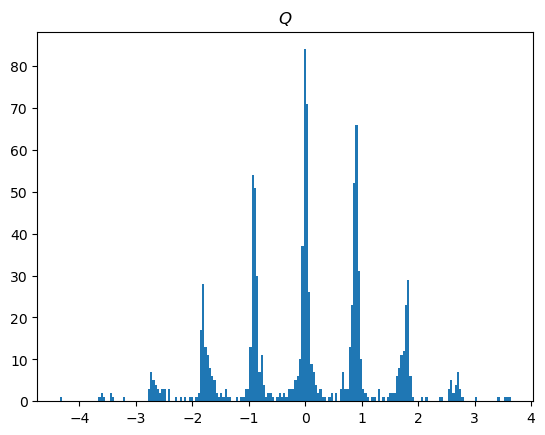
\includegraphics[width=\linewidth]{images/istoB1.png}
    \caption{Reticolo B1}
  \end{subfigure}
  \hfill
  \begin{subfigure}{0.41\linewidth}
    \centering
    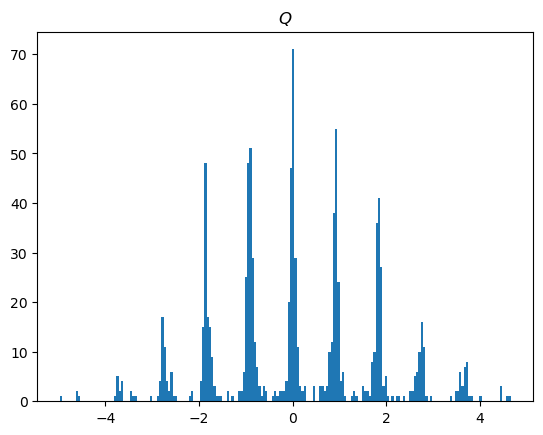
\includegraphics[width=\linewidth]{images/istoB2.png}
    \caption{Reticolo B2}
  \end{subfigure}
  \hfill
  \begin{subfigure}{0.41\linewidth}
    \centering
    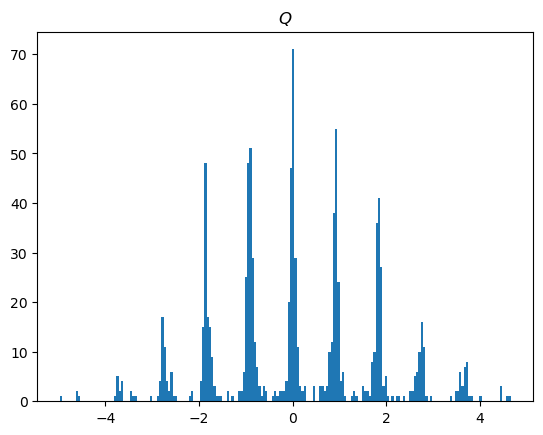
\includegraphics[width=\linewidth]{images/istoB2.png}
    \caption{Reticolo B3}
  \end{subfigure}
  \caption{Distribuzione della carica topologica con 200 bin.}
  \label{isotrgrammi}
\end{figure}

Sappiamo che la larghezza degli istogrammi, ovvero la media di $Q^2$ è la suscettività topologica che vogliamo calcolare. Dagli istogrammi notiamo come la carica topologica si concentri attorno ai valori interi, ovvero i valori che può assumere nel continuo. La larghezza dei picchi attorno ai valori interi è dovuta agli errori di discretizzazione, infatti nei tre reticoli notiamo una larghezza dei picchi che tende a diminuire con il diminuire del passo reticolare. \\ 
Per calcolare l'errore statistico sulla media di $Q^2$ possiamo utilizzare il teorema del limite centrale, a patto che le varie estrazioni di $Q$ siano scorrelate tra di loro. Per verificare che questo è il caso andiamo a calcolare la funzione di autocorrelazione $\Gamma(t_M)$, che quantifica il livello di correlazione delle osservabili ed definita come 
\begin{equation}
    \Gamma(t_M)=\mathbb{E}[Q_i\,Q_{i+t_M}]-\left(\mathbb{E}[Q]\right)^2.
\end{equation}
Il risultato è rappresentato in Figura \ref{Gamma}. Come si osserva la funzione decade velocemente a zero, a conferma che possiamo considerare le variabili come scorrelate.

\begin{figure}[h]
    \centering
    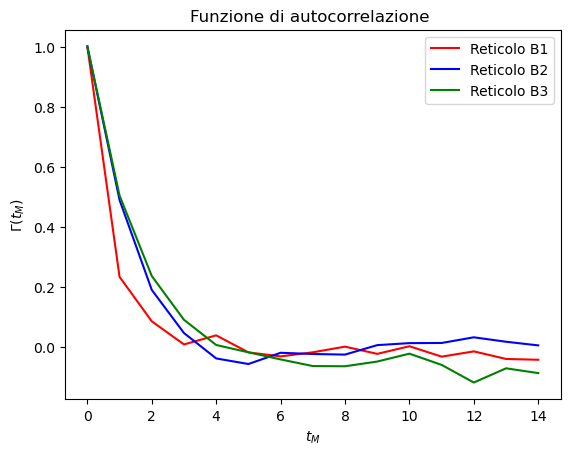
\includegraphics[width=0.8\textwidth]{images/gamma.png}
    \caption{Funzione di autocorrelazione $\Gamma$ per la carica topologica per i tre reticoli considerati. La funzione è normalizzata in modo che $\Gamma(0)=1$. }
    \label{Gamma}
\end{figure}

Riportiamo in Tabella \ref{susc} i risultati della media di $Q^2$ nei 3 reticoli, con l'errore che è stato calcolato usando il teorema del limite centrale. 

\begin{table}[h]
    \centering
    \begin{tabular}{||c c||} 
     \hline
     Reticolo & $\left< Q^2\right>$ \\[0.5ex] 
     \hline\hline
     B1 & $ 1.61 \pm 0.07$  \\
     B2 & $2.84 \pm 0.08$  \\
     B3 & $1.66 \pm 0.08$  \\[1ex] 
     \hline
    \end{tabular}
    \caption{Valori di $\langle Q^2 \rangle$ misurati nei 3 reticoli.}
    \label{susc}
\end{table}

Per ottenere il valore della suscettività topologica nel continuo effettuiamo un fit lineare di $t_0^2\,\chi$ al variare di $a^2/t_0$. Il termine noto sarà il risultato nel continuo cercato. I risultati del fit sono rappresentati in Tabella \ref{tab:estrapolazione} e Figura \ref{fig:estrapolazione}.

\begin{figure}[h]
    \centering
    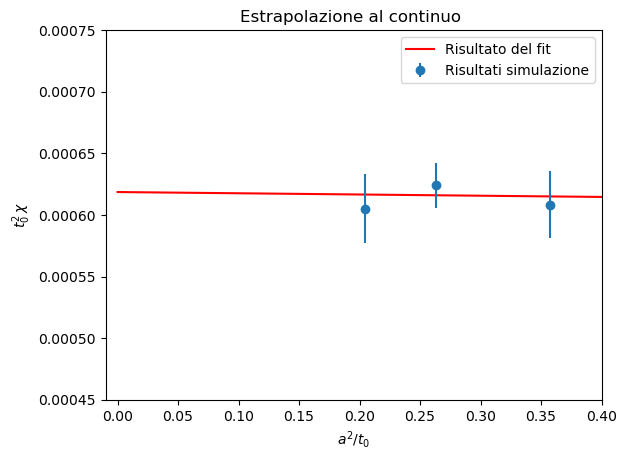
\includegraphics[width=0.8\textwidth]{images/estrapolazione.png}
    \caption{Estrapolazione al continuo della suscettività topologica.}
    \label{fig:estrapolazione}
\end{figure}

\begin{table}[h]
    \centering
    \begin{tabular}{||c c||} 
     \hline
     $t_0^2 \,\chi$ & $\chi^2$ ridotto \\[0.5ex] 
     \hline\hline
     $(6.2\pm0.7)\times 10^{-4}$ & $0.4$ \\[1ex] 
     \hline
    \end{tabular}
    \caption{Risultanti del fit dell'estrapolazione al continuo.}
    \label{tab:estrapolazione}
\end{table}



Il risultato può anche essere convertito in unità fisiche, fornendo il valore
\begin{equation}
    \chi=(177\pm5\pm4\,\textup{MeV})^4,
\end{equation}
dove il primo errore mostrato è un errore statistico, mentre il secondo è sistematico. 

Utilizzando la (\ref{witten Veneziano}) possiamo ora calcolare la massa del mesone $\eta'$ ottenendo 
\begin{equation}
    m_{\eta'}=(927  \pm  40)\,\textup{MeV},
\end{equation}
che risulta compatibile con il valore sperimentale di $957.6(6)\,\textup{MeV}$.


\section{Conclusione}
Il calcolo della suscettività topologica in QCD risulta importante per via del meccanismo di Witten-Veneziano, che la lega alla massa del mesone $\eta'$. La suscettività può essere calcolata a partire da varie estrazioni dalla carica topologica come suo secondo cumulante. In questo lavoro abbiamo ottenuto estrazioni indipendenti della carica topologica tramite simulazioni su reticolo a vario passo reticolare, che ci ha permesso di effettuare una estrapolazione per trovare la suscettività topologica nel continuo. La miglior stima ottenuta è $$\chi=(177\pm5\pm4\,\textup{MeV})^4.$$










\end{document}
